\documentclass[10pt,letterpaper]{article}

\usepackage{color}
\usepackage{amsmath}
\usepackage{float}
\usepackage{placeins}
\usepackage{mathtools,xparse}
\usepackage{cite}
\usepackage{graphicx}
\usepackage[T1]{fontenc}


\DeclarePairedDelimiter{\abs}{\lvert}{\rvert}
\newcommand{\bigCI}{\mathrel{\text{\scalebox{1.07}{$\perp\mkern-10mu\perp$}}}}
\DeclareMathOperator*{\argmax}{arg\,max} 
%%%%%%%%%%%%%%%%%%%%%%% begin %%%%%%%%%%%%%%%%%%%%%%%%%%%%%%
\begin{document}
\pagenumbering{arabic}
\title{Analytic continuation of quantum Monte Carlo data via maximum entropy method}
\author{Michael Haslauer, Max Weber}

%%%%%%%%%%%%%%%%%%%%%%% References %%%%%%%%%%%%%%%%%%%%%%%%%
% \begin{thebibliography}{99}

% \end{thebibliography}
%%%%%%%%%%%%%%%%%%%%%%%%%%  body  %%%%%%%%%%%%%%%%%%%%%%%%%%
\section{Introduction} % (fold)
\label{sec:introduction}

% section introduction (end)
\section{Theory} % (fold)
\label{sec:theory}

% section theory (end)
\newpage
\section{Numerical algorithm} % (fold)
\label{sec:numerical_algorithm}
In this section we describe the numerical algorithm to perform the analytic continuation of quantum Monte Carlo data by the maximum entropy method. As described in Sec. \ref{sec:theory} the quantity $Q = \alpha S - L$ has to be maximized with respect to $\vec A$ in order to find the most probable $\vec A$ given the noisy Greens function $\vec G$. To maximize Q we calculate the gradient of Q with respect to $\vec A$ and set it to zero:
\begin{equation}
	\vec\nabla Q =  \alpha \vec\nabla S - \vec\nabla L = 0
	\label{numerical_algorithm:equ.1}
\end{equation}
Then Equ. \ref{numerical_algorithm:equ.1} leads to:
\begin{equation}
	- \alpha \log \bigg(\frac{A_i}{m_i} \bigg) = \sum K_{ji} \frac{\partial L}{\partial \vec F}
	\label{numerical_algorithm:equ.2}
\end{equation}
where:
\begin{equation}
	\vec F = \mathbf{K} \vec A \text{ and } \vec \nabla L = \frac{\partial \vec F}{\partial \vec A} \frac{\partial L}{\partial \vec F} = \mathbf{K}^T \frac{\partial L}{\partial \vec F}
	\label{numerical_algorithm:equ.3}
\end{equation}
The solution $\vec A$ to the problem can then be represented in terms of a vector $\vec v$
\begin{equation}
	\log \bigg(\frac{\vec A}{\vec m}\bigg) = \mathbf{K}^T \vec v
	\label{numerical_algorithm:equ.4}
\end{equation}
where Equ. \ref{numerical_algorithm:equ.4} has to be read component wise.
Now, a singular value decomposition of $\mathbf{K}$ is performed with $\mathbf{K} = \mathbf{V} \mathbf{\Sigma} \mathbf{U}^T$. Please note that both $\mathbf{V}$ and $\mathbf{U}$ are orthonormal matrices and therefor $\mathbf{V}^{-1}=\mathbf{V}^T$ and $\mathbf{U}^{-1}=\mathbf{U}^T$.
Here $\mathbf{\Sigma}$ has only nonzero components on its diagonal which are called the singular values of $\mathbf{K}$. Because $\mathbf{K}^T$ and $\mathbf{U}$ share the same vector space the solution $\vec A$ can also be represented by a new vector $\vec u$
\begin{equation}
	A_i = m_i \exp \Big(\sum U_{in}u_n\Big)
	\label{numerical_algorithm:equ.5}
\end{equation}
Now Bryan argues that unless $\mathbf{K}$ is of full rank the components of $\vec u$ will not be independent.
Because of the limited precision of the computer and the singular value decomposition some of the singular values of $\mathbf{K}$ will effectively be zero. The search for the optimal $\vec u$ can therefor be reduced to the nonzero singular values of $\mathbf{K}$. Let $s$ be the number of nonzero singular values the search can then be limited to the $s$-dimensional space which Bryan calls the singular space.
Bryan's method therefor first reduces all relevant matrices to the singular space. The vector $\vec u$ is now of length $s$, the number of columns of $\mathbf{V}$ and $\mathbf{U}$ are reduced to $s$ and $\mathbf{\Sigma}$ is now a $s \times s$ square matrix. Making use of Equ. \ref{numerical_algorithm:equ.5} and $\mathbf{K} = \mathbf{V} \mathbf{\Sigma} \mathbf{U}^T$ Equ. \ref{numerical_algorithm:equ.2} can be rewritten as:
\begin{equation}
	-\alpha \mathbf{U} \vec u = \mathbf{U} \mathbf{\Sigma} \mathbf{V}^T \frac{\partial L}{\partial \vec F}
	\label{numerical_algorithm:equ.6}
\end{equation}
Multiplying Equ. \ref{numerical_algorithm:equ.6} by $\mathbf{U}^T$ on both sides it reduces to
\begin{equation}
	-\alpha \vec u = \mathbf{\Sigma} \mathbf{V}^T \frac{\partial L}{\partial \vec F} \equiv g 
	\label{numerical_algorithm:equ.7}
\end{equation}
or
\begin{equation}
	-\alpha \vec u - g = 0
	\label{numerical_algorithm:equ.8}
\end{equation}
Equ. \ref{numerical_algorithm:equ.8} can be solved by a multidimensional Newton search iteratively
\begin{equation}
	\mathbf{J} \vec{\delta u} = -\alpha \vec u - g
	\label{numerical_algorithm:equ.9}
\end{equation}
where $\mathbf{J} = \alpha \mathbf{I} + \frac{\partial \vec g}{\partial \vec u}$ is the Jacobian and $\mathbf{I}$ the identity matrix. 
With $\mathbf{W} = \frac{\partial^2 L}{\partial^2 \vec F}$, $\mathbf{M} = \mathbf{\Sigma}\mathbf{V}^T\mathbf{W}\mathbf{V}\mathbf{\Sigma}$ and $\mathbf{T} = \mathbf{U}^T \vec A \mathbf{U}$ Equ. \ref{numerical_algorithm:equ.9} reads
\begin{equation}
	((\alpha + \mu) \mathbf{I} + \mathbf{M}\mathbf{T}) \vec{\delta u} = -\alpha \vec u - g
	\label{numerical_algorithm:equ.10}
\end{equation}
At each iteration step of the Newton search the step length $\vec{\delta u}$ muss be restricted for the stability of the algorithm.
Therefor, also a Levenberg-Marquardt parameter $\mu$ is added in Equ.\ref{numerical_algorithm:equ.10} to ensure stability.
Bryan proposes $\vec{\delta u}^T T \vec{\delta u} \leq \sum m_i$ as a maximum step length for the algorithm.
However, we found that sometimes even if this criterion is fulfilled the algorithm can be instable due to numerical overflow in Equ. 5.
Therefor, we use the criterion $\parallel \vec A \parallel^2 \leq \sum_i m_i$.
The Newton search can be made more efficient by diagonalizing Equ. \ref{numerical_algorithm:equ.10}. First we diagonalize $\mathbf{T}$:
\begin{equation}
	\begin{gathered}
		\mathbf{T} \mathbf{P} = \mathbf{P} \mathbf{\Gamma},\\
		\mathbf{\Gamma} = \mathbf{diag} \{\gamma_i\}
	\end{gathered}
	\label{numerical_algorithm:equ.11}
\end{equation}
Then we define
\begin{equation}
	\mathbf{B} = \mathbf{diag} \{ \gamma_i^{\frac{1}{2}}\}\mathbf{P}T \mathbf{M}\mathbf{P}\mathbf{diag}\{ \gamma_i^{\frac{1}{2}}\}
	\label{numerical_algorithm:equ.12}
\end{equation}
and again solve the eigenvalue equation
\begin{equation}
	\begin{gathered}
		\mathbf{B} \mathbf{R} = \mathbf{R} \mathbf{\Lambda},\\
		\mathbf{\Lambda} = \mathbf{diag} \{\lambda_i\}
	\end{gathered}
	\label{numerical_algorithm:equ.13}
\end{equation}
Please note that $\mathbf{P}$ and $\mathbf{R}$ are orthogonal matrices and $\gamma_i$ and $\lambda_i$ the eigenvalues of $\mathbf{T}$ and $\mathbf{B}$. Then to finally diagonalize Equ. \ref{numerical_algorithm:equ.10} we define 
\begin{equation}
	\mathbf{Y} = \mathbf{P} \mathbf{diag}\{ \gamma_i^{\frac{1}{2}}\} \mathbf{R}
	\label{numerical_algorithm:equ.14}
\end{equation}
With $\mathbf{Y}^{-T}\mathbf{Y}^{-1} = \mathbf{T}$ and $\mathbf{Y}^{-1}\mathbf{M}\mathbf{Y}^{-T} = \mathbf{\Lambda}$ Equ. \ref{numerical_algorithm:equ.10} can be rewritten as
\begin{equation}
	[( \alpha + \mu) \mathbf{I} +\mathbf{\Lambda}]\mathbf{Y}^{-1} \vec{\delta u} = \mathbf{Y}^{-1}[ -\alpha \vec u - \vec g]
	\label{numerical_algorithm:equ.15}
\end{equation}
which leads to s independent equations for $\mathbf{Y}^{-1} \vec{\delta u}$.
Now Equ. \ref{numerical_algorithm:equ.10} can be rewritten to
\begin{equation}
	(\alpha + \mu)\vec{\delta u} = -\alpha \vec u - g - \mathbf{M}\mathbf{Y}^{-T}\mathbf{Y}^{-1} \vec{\delta u}
	\label{numerical_algorithm:equ.16}
\end{equation}
So to finally we first solve Equ. \ref{numerical_algorithm:equ.15} for $\mathbf{Y}^{-1} \vec{\delta u}$, use it in Equ. \ref{numerical_algorithm:equ.16} to solve for $\vec{\delta u}$ and calculate the new value for $\vec u_{n+1} = \vec u_{n} + \vec{\delta u}$. The iteration is terminated if $\sum_i |\vec u_{n+1} - \vec u_{n}| \leq 10^{-10}$.
% section numerical_algorithm (end)
\section{Results} % (fold)
\label{sec:results}
In this section we investigate the performance of the Maximum entropy method by applying it to synthetic Greens function in order to recover the spectrum $A(\omega)$. We generate the Greens function data by first calculating the spectrum $A(\omega)$ and then using Equ. to calculate the Greens function given our spectrum and the kernel $K(\tau,\omega)$. After that we corrupt the Greens function by Gaussian noise as the ``real'' Greens function obtained by Quantum Monte Carlo methods always suffer from noise. In this evaluation we solely use the spectrum of the BCS superconductor for our investigation which can be calculated by 
\begin{equation}
	A(\omega) = 
		\begin{cases}
			\frac{1}{W} \frac{|\omega|}{\sqrt{\omega^2 - \Delta^2}}&, \text{ if } \Delta < |\omega| < \frac{W}{2} \\
			0 &, \text{else}
		\end{cases}
	\label{results:equ.1}
\end{equation}
where $W$ denotes the bandwidth and $2\Delta$ the gap magnitude.
In Fig. we show an example of the spectrum and the resulting Greens function for $W = 0.9$ and $\Delta = 10$.
\begin{figure}[htbp]
	\centering
	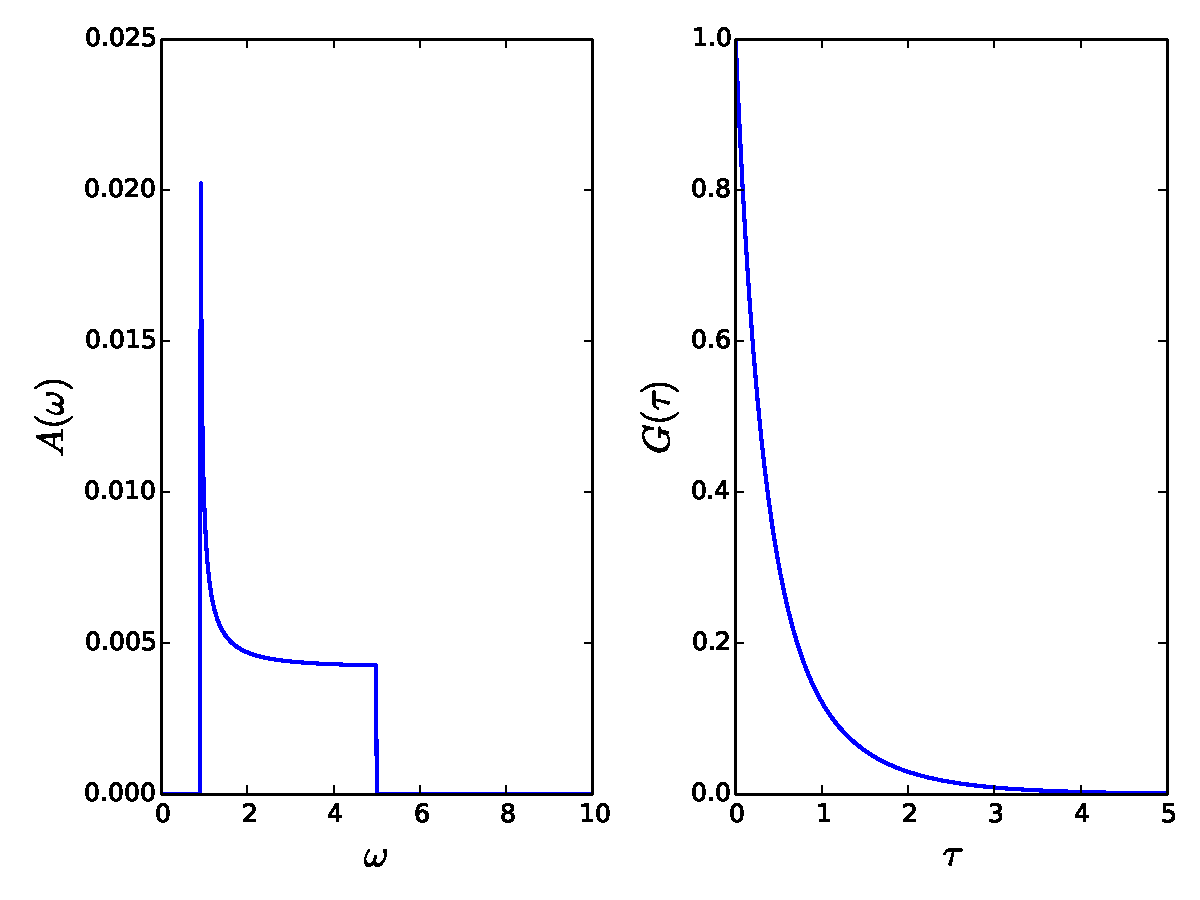
\includegraphics[width=0.95\textwidth]{./images/BCS_A_G_example.pdf}
	\caption{Example BCS spectrum $A(\omega)$ (left) and resulting Greens function $G(\tau)$ (right). The spectrum is calculated according to Equ. \ref{results:equ.1} with $\Delta = 0.9$ and $W = 10$.}
	\label{results:fig.1}
\end{figure}
\FloatBarrier
The results obtained by Maximum entropy highly depend on the regularization parameter $\alpha$. We demonstrate the influence of $\alpha$ by estimating the spectrum shown in Fig. \ref{results:fig.1} for three different values for $\alpha = 0.5,2.5,10$. The results are shown in Fig. \ref{results:fig.2}
\begin{figure}[htbp]
	\centering
	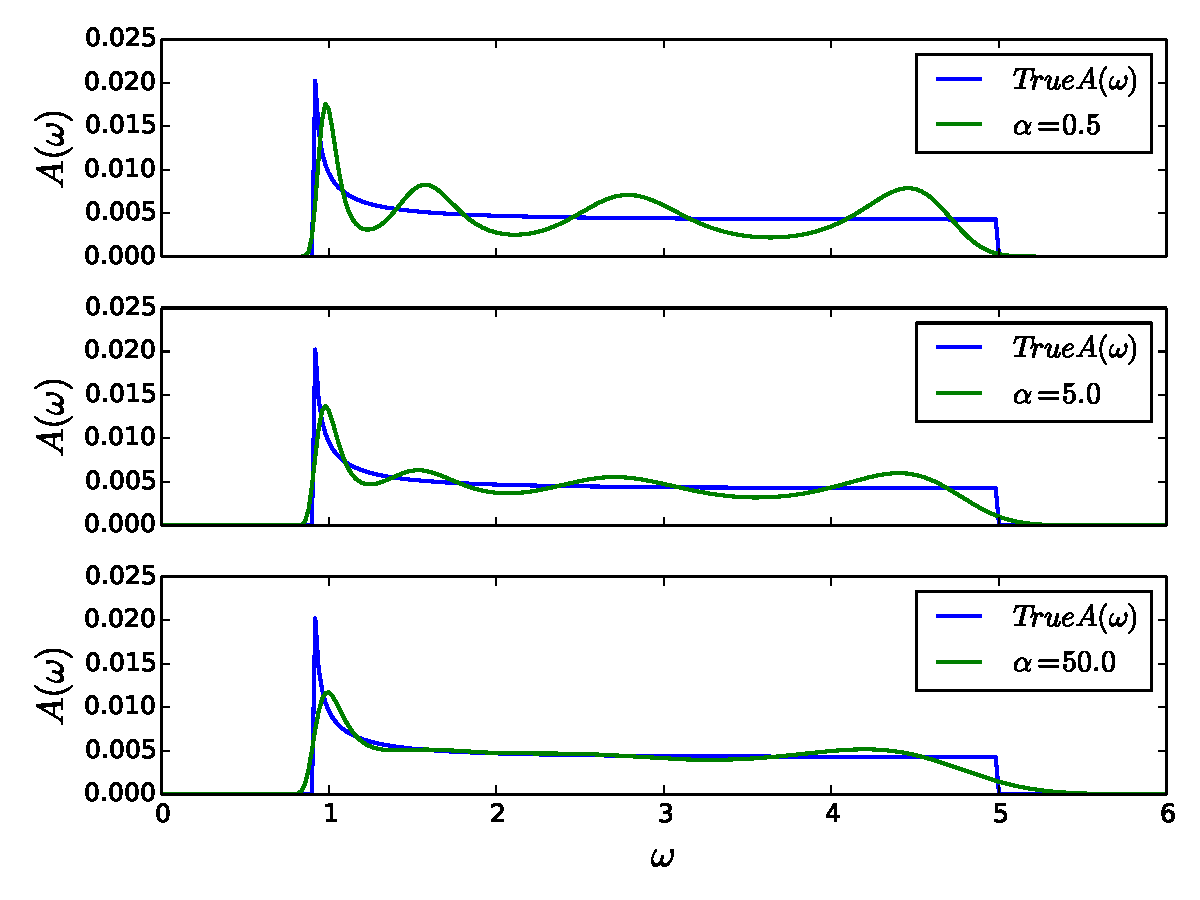
\includegraphics[width=0.95\textwidth]{./images/BCS_varying_alpha.pdf}
	\caption{Influence of the regularization parameter $\alpha$ on the performance of the Maximum Entropy method. The spectrum is calculated according to Equ. \ref{results:equ.1} with $\Delta = 0.9$ and $W = 10$.}
	\label{results:fig.2}
\end{figure}
\FloatBarrier
Another important parameter is the choice of the minimum singular value $\theta$ which determines the dimension of the singular space. We investigate the impact of $\theta$ on the performance of the Maximum Entropy method in Fig. \ref{results:fig.3}
\begin{figure}[htbp]
	\centering
	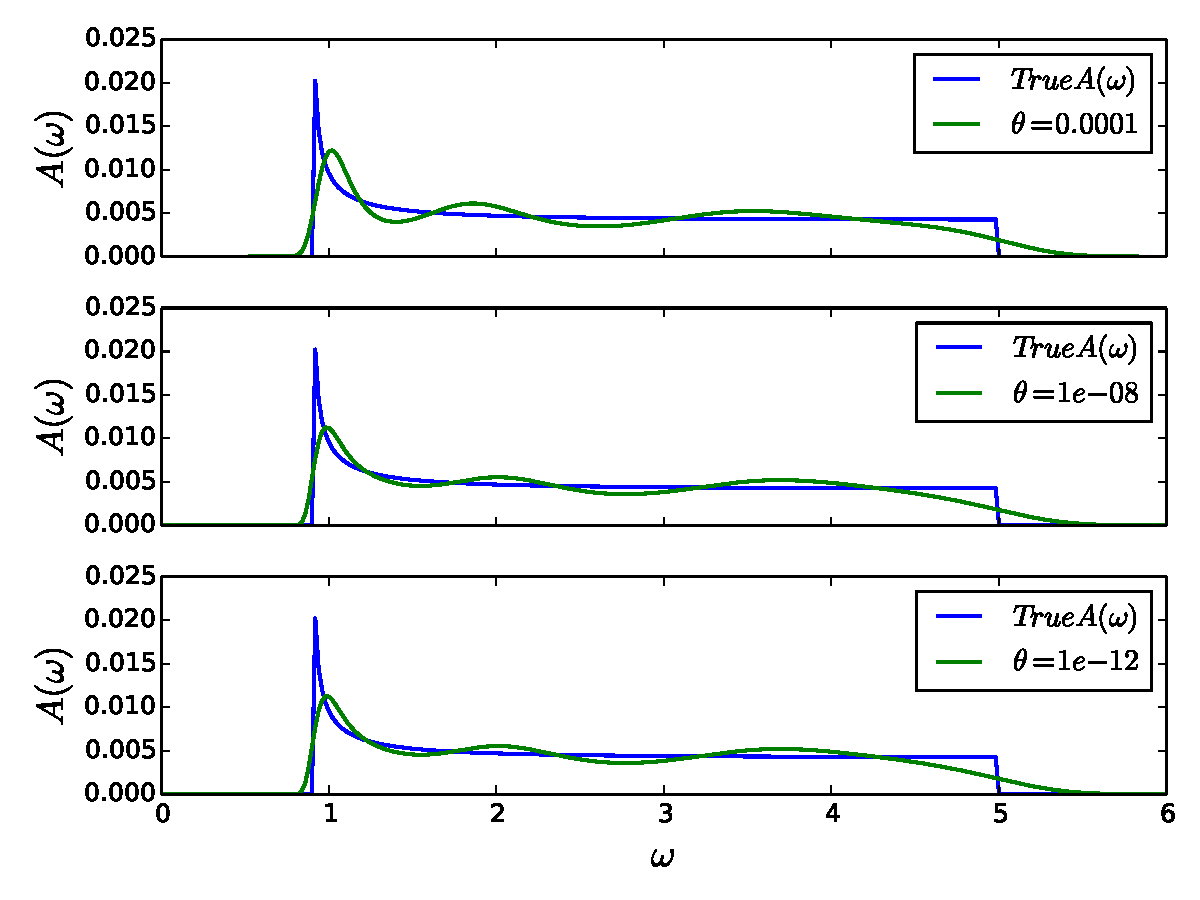
\includegraphics[width=0.95\textwidth]{./images/BCS_varying_cutoffs.pdf}
	\caption{Influence of the minimum singular value $\theta$ on the performance of the Maximum Entropy method. The spectrum is calculated according to Equ. \ref{results:equ.1} with $\Delta = 0.9$ and $W = 10$.}
	\label{results:fig.3}
\end{figure}
\FloatBarrier
% section results (end)
\section{Conclusions} % (fold)
\label{sec:conclusions}
% section conclusions (end)
\end{document}
